% ---
% filename : ["electrotechnique_circuits_dc_20260429_420_pente_loi_ohm.tex"]
% id : "electrotechnique_circuits_dc_20260429_420"
% title : "Pente et interprétation physique de la loi d'Ohm"
% domain : "Électrotechnique"
% subdomain : "Circuits DC"
% tags : ["loi d'Ohm", "résistance", "pente", "tangente", "caractéristique", "ts"]
% difficulty : 2
% time_solve : 16  # Calcul : 2 (difficulté) * (4 questions * 2)
% has_octave : true
% octave_files : ["electrotechnique_circuits_dc_20260429_420_pente_loi_ohm.m"]
% author : "om"
% ---
\documentclass[a4paper,11pt,answers,addpoints]{exam}
% ---------------------------------------------------------
% LANGUE, ENCODAGE, FONTS
% ---------------------------------------------------------
\usepackage[utf8]{inputenc}

% ---------------------------------------------------------
% GÉOMÉTRIE ET MISE EN PAGE
% ---------------------------------------------------------
\usepackage[left=1.7cm,right=1.5cm,top=2cm,bottom=1cm]{geometry}
%\usepackage{a4wide}
\usepackage{microtype}      % Meilleure répartition du texte
\usepackage{float}          % Positionnement [H]
\usepackage{needspace}      % Saut conditionnel intelligent

% Éviter les veuves/orphelines (optionnel, à décommenter si besoin)
% \widowpenalty=10000
% \clubpenalty=10000

% Espacement vertical flexible
%\raggedbottom
%\setlength{\parskip}{0.5em plus 0.2em minus 0.1em}
%\setlength{\parindent}{0pt}


% ---------------------------------------------------------
% MATHÉMATIQUES
% ---------------------------------------------------------
\usepackage{amsmath, amssymb, bm, esvect}

% Vecteurs
\newcommand{\V}{\overrightarrow}
\def\vect#1{\overrightarrow{\strut#1}}
\providecommand{\Degrees}[0]{\ensuremath{^\circ}}

% ---------------------------------------------------------
% UNITÉS ET GRANDEURS (SIunitx)
% ---------------------------------------------------------
\usepackage{siunitx}
\sisetup{output-decimal-marker={,}}
\DeclareSIUnit \var {var}
\DeclareSIUnit \VA {VA}
\DeclareSIUnit \kVA {kVA}
\DeclareSIUnit[quantity-product={}] \degree{\text{\textdegree}}

% ---------------------------------------------------------
% GRAPHIQUES : TikZ + CircuitikZ + PGFPlots
% ---------------------------------------------------------
\usepackage{tikz}
\usetikzlibrary{
	arrows.meta,
	intersections,
	decorations.pathreplacing,
	positioning
}

\usepackage[european,straightvoltages,EFvoltages]{circuitikz}

\usepackage{tkz-fct}
\usepackage{pgfplots}
\pgfplotsset{compat=1.12}

% Symbole étoile-triangle personnalisé
\newcommand{\wye}{%
	\mathbin{\tikz[x=1ex,y=1ex]{%
			\draw[line width=.1ex] (0,0)--(45:1)--++(-45:1) (45:1)--++(0,1);
	}}%
}


\usepackage{sankey}

\pgfdeclarelayer{background}
\pgfdeclarelayer{foreground}
\pgfdeclarelayer{sankeydebug}
\pgfsetlayers{background,main,foreground,sankeydebug}


% ---------------------------------------------------------
% TABLEAUX
% ---------------------------------------------------------
\usepackage{tabularx}
\usepackage{tabu}

% ---------------------------------------------------------
% HYPERLIENS
% ---------------------------------------------------------
\usepackage[colorlinks=true,
menucolor=red,
breaklinks=true,
urlcolor=blue,
linkcolor=blue]{hyperref}

% ---------------------------------------------------------
% COMMANDES PERSONNELLES
% ---------------------------------------------------------
\newcommand\nomauteur{bdminasmorgul@protonmail.com}
\newcommand\dateTe{29.04.2026}
\newcommand\brancheTe{TS}

% ---------------------------------------------------------
% STYLE DE L'EXERCICE
% ---------------------------------------------------------
\pagestyle{headandfoot}
\firstpageheadrule
\runningheadrule

\firstpageheader{\brancheTe\ (\nomauteur)}{Élève : }{(\dateTe) \thepage/\numpages}
\runningheader{\brancheTe\ (\nomauteur)}{Élève : }{(\dateTe) \thepage/\numpages}

% Compteur en bas de page
\newcommand{\totalpointtts}{%
	\begin{tikzpicture}[remember picture, overlay]
		\node[anchor=south west, inner sep=0pt, outer sep=0pt]
		at ([xshift=0.5cm,yshift=0.5cm]current page.south west)
		{\rotatebox{90}{Total des points : \numpoints}};
	\end{tikzpicture}
}

\firstpagefooter{\totalpointtts}{}{}
\runningfooter{\totalpointtts}{}{}

% Réglages exam
\printanswers
\addpoints
\pointsinmargin
\bracketedpoints

% ---------------------------------------------------------
% LISTINGS (code)
% ---------------------------------------------------------
\usepackage{xcolor}
\usepackage{listings}

\lstdefinestyle{octavestyle}{
	language=Matlab,
	basicstyle=\ttfamily\small,
	keywordstyle=\color{blue},
	commentstyle=\color{green!50!black},
	stringstyle=\color{red},
	stepnumber=1,
	frame=single,
	breaklines=true,
	breakatwhitespace=true,
	tabsize=4
}
\usepackage{enumitem}
% Réglage global : toutes les listes enumerate (niveau 1) en a), b), c), ...
\setlist[enumerate,1]{label=\alph*), ref=\alph*)}
\newenvironment{explication}{%
	\par\noindent\textbf{Explication. }\itshape
}{\par\normalfont}


%\renewcommand{\thepartno}{\arabic{partno}}
%\renewcommand{\partlabel}{\thepartno)}
\begin{document}
\unframedsolutions
\pointsinmargin
\bracketedpoints
\section*{Préparation TS PQ CFC ELMO,IELE,PELE}
\begin{questions}
\question Tracer sur le graphique suivant~:\
\begin{parts}
	\part[3] La résistance $R_1 = \qty{500}{[\ohm]}$
	\begin{solution}
		\begin{align*}
			R_1 &= \qty{500}{[\ohm]}\\
			&\text{On doit avoir 2 points pour tracer une droite}\\
			&\text{Le point 1, c'est (0,0)}\\
			&\text{Le point 2, il faut calculer un couple de coordonnées sur le graphique}\\
			U_{R1} &= R_1 \cdot I_{R1} = \qty{500}{[\ohm]} \cdot \qty{14}{[\milli\ampere]} = \qty{7}{[\volt]}
		\end{align*}
	\end{solution}
	\part[3] La résistance $R_2 = \qty{2000}{[\ohm]}$
	\begin{solution}
		\begin{align*}
		R_2 &= \qty{2000}{[\ohm]}\\
		&\text{On doit avoir 2 points pour tracer une droite}\\
		&\text{Le point 1, c'est (0,0)}\\
		&\text{Le point 2, il faut calculer un couple de coordonnées sur le graphique}\\
		U_{R2} &= R_2 \cdot I_{R2} = \qty{2000}{[\ohm]} \cdot \qty{6}{[\milli\ampere]} = \qty{12}{[\volt]}
		\end{align*}
	\end{solution}
	\part[3] Calculer la pente de la droite qui représente $R_1$
	\begin{solution}
		Voir ci-dessous \pageref{expl:pente}(\ref{expl:pente}) l'explication du calcul de la pente de la droite $R_1$\\
		\[
		\text{Pente de } R_1 = 500 \ \text{donc} \ R_1 = \qty{500}{[\ohm]}
		\]
	\end{solution}
	\part[3] Calculer la pente de la droite qui représente $R_2$
	\begin{solution}
		Voir ci-dessous l'explication du calcul de la pente de la droite $R_2$\\
		\[
		\text{Pente de } R_2 = 2000 \ \text{donc} \ R_2 = \qty{2000}{[\ohm]}
		\]
	\end{solution}
\end{parts}
\begin{center}
	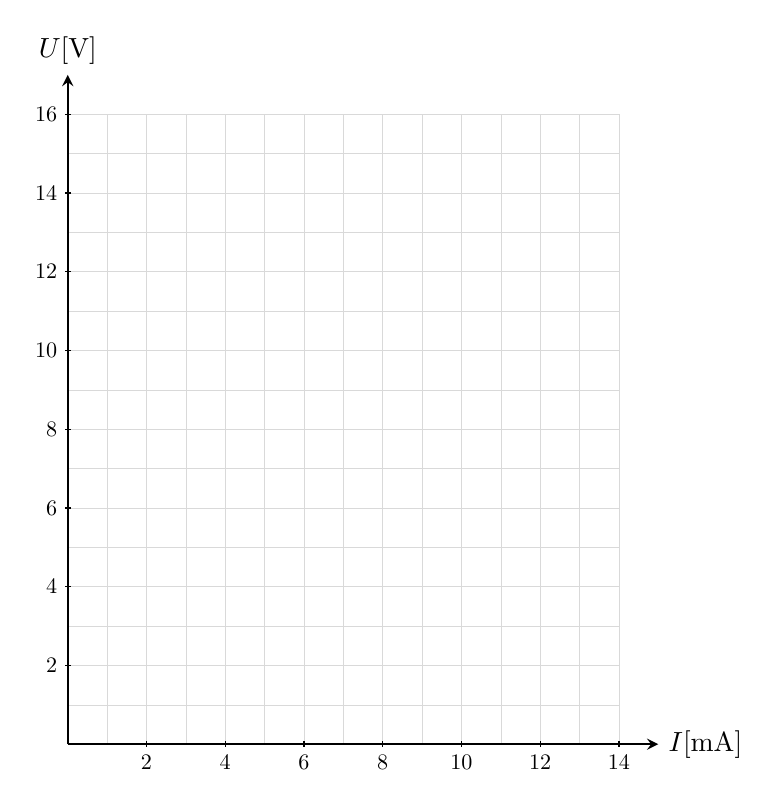
\begin{tikzpicture}[european, >=stealth]
		% Grille
		\draw[step=0.5, gray!30, very thin] (0,0) grid (7,8);
		
		% Axes : I horizontal, U vertical
		\draw[thick, ->] (0,0) -- (7.5,0)
		node[right] {$I \qty{}{[\milli\ampere]}$};
		\draw[thick, ->] (0,0) -- (0,8.5)
		node[above] {$U \qty{}{[\volt]}$};
		
		% Graduations sur I (axe horizontal) : 2,4,...,14 mA
		\foreach \x in {2,4,6,8,10,12,14}
		\draw (\x/2, 1pt) -- (\x/2, -1pt)
		node[below, scale=0.8] {\x};
		
		% Graduations sur U (axe vertical) : 2,4,...,16 V
		\foreach \y in {2,4,6,8,10,12,14,16}
		\draw (1pt, \y/2) -- (-1pt, \y/2)
		node[left, scale=0.8] {\y};
		
		%	\draw[thick, blue] (0,0) -- (7,3.5) node[right] {$R_1$};
		%	\filldraw[blue] (8/2, 8/2) circle (1.5pt);
		%	\draw[thick, red] (0,0) -- (4,8) node[above] {$R_2$};
		%	\filldraw[red] (4/2, 8/2) circle (1.5pt);
	\end{tikzpicture}
\end{center}

%\vspace{0.5em}
%\needspace{50\baselineskip}

%\vspace{4cm}
\needspace{10\baselineskip}

\begin{solution}
\begin{center}
	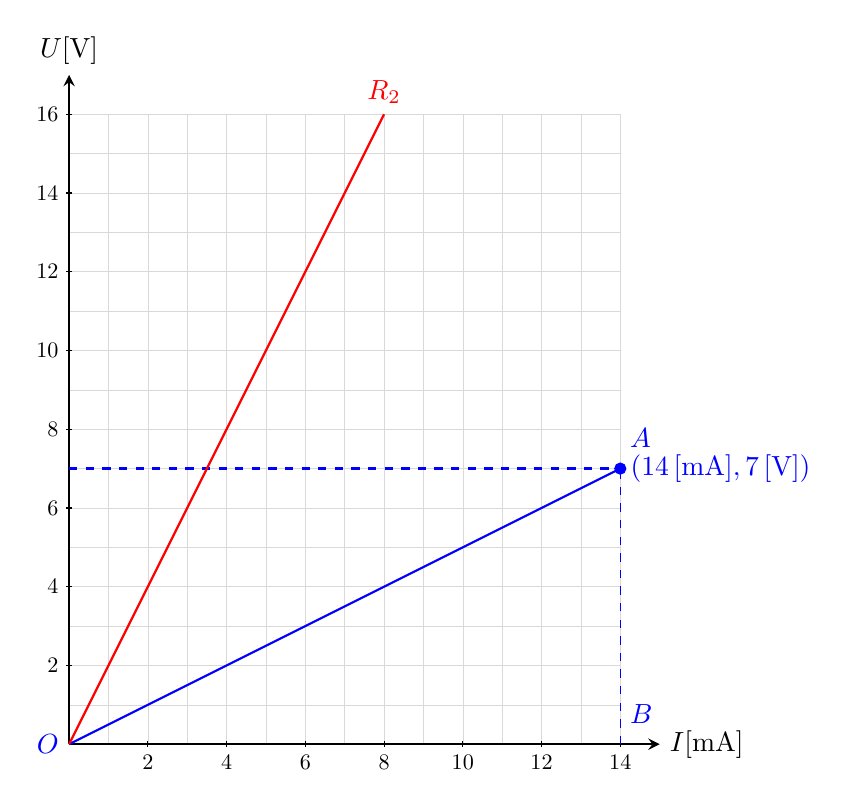
\begin{tikzpicture}[european, >=stealth]
		% Grille
		\draw[step=0.5, gray!30, very thin] (0,0) grid (7,8);
		
		% Axes : I horizontal, U vertical
		\draw[thick, ->] (0,0) -- (7.5,0)
		node[right] {$I \qty{}{[\milli\ampere]}$};
		\draw[thick, ->] (0,0) node[blue,left]{$O$} -- (0,8.5)
		node[above] {$U \qty{}{[\volt]}$};
		
		% Graduations sur I (axe horizontal) : 2,4,...,14 mA
		\foreach \x in {2,4,6,8,10,12,14}
		\draw (\x/2, 1pt) -- (\x/2, -1pt)
		node[below, scale=0.8] {\x};
		
		% Graduations sur U (axe vertical) : 2,4,...,16 V
		\foreach \y in {2,4,6,8,10,12,14,16}
		\draw (1pt, \y/2) -- (-1pt, \y/2)
		node[left, scale=0.8] {\y};
		
		\draw[thick, blue] (0,0) -- (7,3.5) node[right] {$(\qty{14}{[\milli\ampere]},\qty{7}{[\volt]})$};
		\draw[dashed, blue] (7,0) node[above right,yshift=4pt]{$B$} -- (7,3.5) node[above right,yshift=4pt]{$A$};
		\draw[dashed, thick, blue] (0,7/2) -- (7,3.5);
		\filldraw[blue] (14/2, 7/2) circle (2.0pt);
		\draw[thick, red] (0,0) -- (4,8) node[above] {$R_2$};
		%	\filldraw[red] (4/2, 8/2) circle (1.5pt);
	\end{tikzpicture}
\end{center}
%\vspace{0.5em}
%\needspace{16\baselineskip}
%
%\begin{center}
\end{solution}
\begin{solution}
\begin{center}
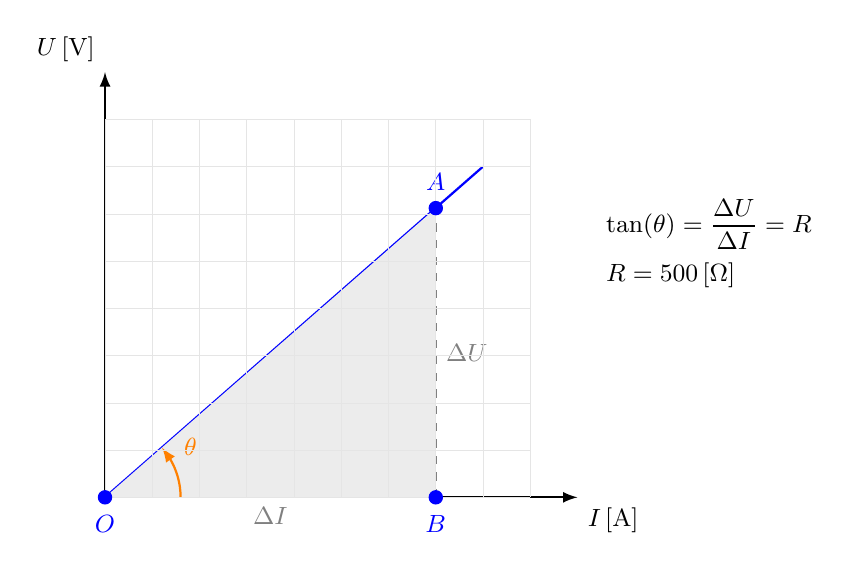
\begin{tikzpicture}[scale=1.2, >=latex, font=\small]
	% Axes
	\draw[->, thick] (0,0) -- (5,0) node[below right] {$I$\,[A]};
	\draw[->, thick] (0,0) -- (0,4.5) node[above left] {$U$\,[V]};
	\draw[blue, thick] (0,0) -- (4,3.5);
	% Point A générique pour le triangle
	\coordinate (O) at (0,0);
	\node[blue, below, yshift=-3pt] at (O) {$O$};
	\coordinate (B) at (3.5,0);
	\node[blue, below, yshift=-3pt] at (B) {$B$};
	\coordinate (A) at (3.5,3.06);
	\node[blue, above, yshift=3pt] at (A) {$A$};
	
	% Triangle rectangle
	\draw[thick, dashed, gray] (B) -- (A) node[midway, right, gray] {$\Delta U$};
	\draw[dashed, gray] (O) -- (B) node[midway, below, gray] {$\Delta I$};
%	\draw[red, thick] (O) -- (A);

	% Remplissage du triangle OBA en gris clair
	\fill[gray!15] (O) -- (B) -- (A) -- cycle;
	% Angle θ
	\draw[->, orange, thick] (0.8,0) arc (0:41:0.8) node[pos=0.6, above right, orange] {$\theta$};
	% Légende tangente
	\node[align=left, anchor=west] at (5.2, 2.5) {
		$\displaystyle \tan(\theta) = \frac{\Delta U}{\Delta I} = R$\\[4pt]
		$\displaystyle R = \qty{500}{[\ohm]}$\\[4pt]
%		\textcolor{gray}{(échelles adaptées)}
	};
	
	% Grille légère pour lisibilité
	\draw[step=0.5, gray!20, very thin] (0,0) grid (4.5,4);

	\filldraw[blue] (O) circle (2.0pt);
	\filldraw[blue] (B) circle (2.0pt);
	\filldraw[blue] (A) circle (2.0pt);
\end{tikzpicture}
\end{center}


\label{expl:pente}\question \textbf{1 : Tangente et pente géométrique sur le papier (sans unité)}

Soit $\theta$ l'angle entre l'axe horizontal $OB$ et la droite $OA$.

Par définition trigonométrique :
\[
\tan(\theta) = \frac{\text{côté opposé}}{\text{côté adjacent}}
= \frac{\Delta y_{\text{[cm]}}}{\Delta x_{\text{[cm]}}} = \dfrac{AB}{OB} = \dfrac{\Delta U}{\Delta I}
\]

Exemple : $\Delta y = \qty{3,5}{\unit{[cm]}}$ et $\Delta x = \qty{5}{[cm]}$, alors
\[
\tan(\theta) = \frac{\qty{3,5}{[cm]}}{\qty{5}{[cm]}} = \num{0.7}
\]

Les cm se simplifient : $\tan(\theta)$ est un \emph{nombre pur} (sans unité).

On peut aussi l'écrire en pourcentage :
\[
p_{\%} = \num{0.7} \cdot 100\% = 70\%.
\]

\vspace{0.5em}
\needspace{5\baselineskip}
\textbf{2 : Interprétation physique sur la loi d'Ohm~: $U = f(I)$}

Sur le graphique $U = f(I)$ :
\[
\tan(\theta) = \frac{\Delta U}{\Delta I}.
\]

Pour le point $A(\qty{14}{[\milli\ampere]},\qty{7}{[\volt]})$~:
\[
\Delta I = \qty{14}{[\milli\ampere]} = \qty{0,014}{[\ampere]}; \qquad
\Delta U = \qty{7}{[\volt]}
\]

Donc
\[
\tan(\theta) = \frac{\qty{7}{}}{\qty{0,014}{}} = \qty{500}{}.
\]

Sur le graphe $U = f(I)$, on a donc
\[
\tan(\theta) = \frac{\Delta U}{\Delta I} = R.
\]

\medskip
\textbf{3 : Lien via les échelles de tracé}

Si l’échelle verticale est $1\ \text{[V/cm]}$ et l’échelle horizontale $2\ \text{[mA/cm]}$ :

\[
R = \tan(\theta)_{\text{papier}} \cdot
\frac{\text{échelle verticale}}{\text{échelle horizontale}}
\]

Par exemple, pour $\tan(\theta)_{\text{papier}} = \num{0.7}$ :
\[
R = \num{0.7} \cdot \frac{1\ \text{[V/cm]}}{\num{0,002}\ \text{[A/cm]}}
= \num{0.7} \cdot 500\ \unit{[\ohm]}
= 350\ \unit{[\ohm]}.
\]

Pour retrouver $R = 500\ \unit{[\ohm]}$ :
\[
\tan(\theta)_{\text{papier}} =
\frac{R \cdot \text{échelle horizontale}}{\text{échelle verticale}}
= \frac{500\ \unit{[\ohm]} \cdot \num{0,002}\ \text{[A/cm]}}{1\ \text{[V/cm]}} = 1
\]

Avec ces échelles, $\theta = 45^\circ$ (car $\tan(\theta) = 1$) et on retrouve $R = 500\ \unit{[\ohm]}$.

\medskip
\textbf{Conclusion :} $\tan(\theta)$ fait le lien entre géométrie et physique :
sur le papier, c’est un \emph{rapport de longueurs} (sans unité) alors que sur le graphique $U = f(I)$,
\[
\tan(\theta) = \frac{\Delta U}{\Delta I} = R\ \unit{[\ohm]}.
\]

\vspace{0.5em}
\needspace{15\baselineskip}
\begin{verbatim}
	% Télécharger OCTAVE depuis [https://wiki.octave.org/Using_Octave]
	% et l'installer. Puis copier-coller le code dans OCTAVE.
	% === Étape 4 : Tangente, pente et résistance R ===
	% Données du point A : U = 7 V, I = 14 mA
	U_A = 7;            % [V]
	I_A_mA = 14;        % [mA]
	I_A = I_A_mA / 1000;% [A] conversion
	
	% --- Résistance directe (méthode recommandée) ---
	R_direct = U_A / I_A;
	printf("Point A : U = %.1f [V], I = %.1f [mA]\n", U_A, I_A_mA);
	printf("Resistance R = DeltaU/DeltaI = %.1f [ohm]\n\n", R_direct);
	
	% --- Tangente sur papier (avec échelles) ---
	ech_V_cm = 1;       % [V/cm] verticale
	ech_mA_cm = 2;      % [mA/cm] horizontale
	ech_A_cm = ech_mA_cm / 1000; % [A/cm]
	
	delta_y_cm = U_A / ech_V_cm;
	delta_x_cm = I_A_mA / ech_mA_cm;
	tan_papier = delta_y_cm / delta_x_cm;
	theta_deg = atand(tan_papier);
	
	printf("Pente papier (tan theta) : %.2f (sans unite)\n", tan_papier);
	printf("Angle theta papier : %.1f [degres]\n", theta_deg);
	printf("Pente en % : %.1f %\n\n", tan_papier * 100);
	
	% --- Résistance via échelles ---
	R_echelles = tan_papier * (ech_V_cm / ech_A_cm);
	printf("Resistance via echelles : %.1f [ohm]\n", R_echelles);
	
	% --- Tangente papier requise pour R = 500 ohm ---
	tan_requis = R_direct * ech_A_cm / ech_V_cm;
	theta_requis = atand(tan_requis);
	printf("\nPour R = %.1f [ohm] avec ces echelles :\n", R_direct);
	printf("  Tangente papier requise : %.2f\n", tan_requis);
	printf("  Angle requis : %.1f [degres]\n", theta_requis);
	
	% --- Vérification ---
	if abs(R_echelles - R_direct) < 1e-6
	printf("\nVerification : OK - methodes concordantes.\n");
	else
	printf("\nAttention : échelles non adaptees au point A.\n");
	end		
\end{verbatim}

\end{solution}
\end{questions}
\end{document}


